%  compress using: gs -sDEVICE=pdfwrite -dCompatibilityLevel=1.4 -dNOPAUSE -dQUIET -dBATCH      -sOutputFile=foo-compressed.pdf gradientDescentWirelessNetworks.pdf
% submit at  https://cmt.research.microsoft.com/TXWMCS2015/Default.aspx
% http://texassymposium.org/PaperSubmission.html

\documentclass[conference]{IEEEtran}
\newcommand{\subparagraph}{}
\bibliographystyle{plain}
\usepackage{epsfig,graphicx,cite}
\usepackage{psfrag}
\usepackage[small,compact]{titlesec}
\usepackage{wrapfig}
\usepackage{mathrsfs}
\usepackage{bm}
\usepackage{cite,url,subfigure,epsfig,graphicx}
\usepackage{verbatim,amsfonts,amsmath,amssymb}
\usepackage{fancyhdr}
\usepackage{mathbbold}
\usepackage{bbm}
\usepackage{mathrsfs}
\usepackage{amsfonts}
\usepackage{cite,url,subfigure,epsfig,graphicx}
\usepackage{amssymb,amsmath,bm,makecell}
\usepackage{indentfirst}
\usepackage{overpic}
\newcommand{\figwid}{0.22\columnwidth}

\usepackage{amsmath}
\usepackage{algorithm}
\usepackage[noend]{algpseudocode}



\usepackage{mathtools}
\usepackage[font=footnotesize]{caption}
%\usepackage{amsmath}
%\usepackage{amssymb}
\usepackage{tabulary}
\usepackage{booktabs}
%\usepackage{framed}
%\usepackage{fancyhdr}
%\usepackage[hypertex]{hyperref}
\usepackage[hidelinks]{hyperref}
%\IEEEoverridecommandlockouts
\usepackage{cite,url,subfigure,epsfig,graphicx}
\usepackage{times,verbatim,amsfonts,amsmath,color}
\newtheorem{definition}{\textbf{Definition}}
\newtheorem{lemma}{\textbf{Lemma}}
\newtheorem{proof}{\textbf{Proof}}
\newtheorem{theorem}{\textbf{Theorem}}
\newtheorem{example}{\textbf{Example}}
\newtheorem{proposition}{\textbf{Proposition}}
\newtheorem{remark}{\textbf{Remark}}
\newtheorem{corrolary}{\textbf{Corrolary}}
\newtheorem{ex}{\textbf{EX}}
\usepackage{overpic}
\graphicspath{{./},{./pictures/}}
\setcounter{secnumdepth}{4}
\setcounter{tocdepth}{4}
\usepackage[table,xcdraw]{xcolor}
\newcommand{\todo}[1]{\vspace{5 mm}\par \noindent \framebox{\begin{minipage}[c]{0.98 \columnwidth} \ttfamily\flushleft \textcolor{red}{#1}\end{minipage}}\vspace{5 mm}\par}
\let\labelindent\relax \usepackage{enumitem}


% correct bad hyphenation here
\hyphenation{op-tical net-works semi-conduc-tor}
\begin{document}
%
% paper title
% can use linebreaks \\ within to get better formatting as desired
\title{Using Gradient Descent to Optimize Paths for Sustaining Wireless Sensor Networks } %Data Ferrying and Wireless Recharging of 

% author names and affiliations
% use a multiple column layout for up to three different
% affiliations
\author{\IEEEauthorblockN{Srikanth K. V. Sudarshan and Aaron T. Becker}
\IEEEauthorblockA{Dept.~of Electrical and Computer Engineering\\
University of Houston,\\
 Houston, TX 70004, USA\\
Email: \protect{skvenkatasudarshan@uh.edu}, atbecker@uh.edu}}


% make the title area
\maketitle

\begin{abstract}
A structural-health wireless sensor network (WSN) should last for decades, but traditional disposable batteries cannot sustain such a network. Energy is the major impediment to sustainability of WSNs. Most energy is consumed by (i) wireless transmissions of perceived data, and (ii) long-distance multi-hop transmissions from the source sensors to the sink. This paper explores how to exploit emerging wireless power transfer technology by using robotic unmanned vehicles (UVs) to service the WSNs.  These UVs cut data transmissions from long to short-distances, collect sensed information, and replenish WSN's energy. 
This paper presents path-planning and path optimization algorithms for sustaining WSNs.
%Energy costs due to power transmission are less than the UV's transportation costs. This is true for WSNs spread over large geographic areas, terrain with obstacles, or where transportation costs are high, such as subsea or aerial UVs. 
\end{abstract}
\begin{IEEEkeywords} Wireless sensor networks, wireless recharge, robot, unmanned vehicles \end{IEEEkeywords}



\section{Introduction}
New wireless sensor technologies have enabled wireless sensor networks (WSNs) to proliferate in many different fields (e.g., battlefield surveillance, environmental sensing, biomedical observation)~\cite{AkSu02,RenewSN12,EPRNP05,jTbHCC06}.
Although advances in processing and computing designs can endow sensors with a multitude of sensing modalities (temperature, pressure, light, magnetometer, infrared, etc.), advances in battery technology have been more modest.  Energy constraints on battery-powered sensors limits the sustainability of WSNs. In WSNs, the majority of energy is consumed by (\romannumeral1) wireless transmission of perceived data~\cite{ChTyTNet08,RenewSN12,OBSP09}, and (\romannumeral2) long-distance multi-hop transmissions from source sensors to the sink. Radio transmission and listening dominate power usage, as shown in Fig./~\ref{fig:txenergy}.
Research efforts to address WSN energy concerns have focused on energy conservation~\cite{FbNbRbICC09}, environmental energy harvesting~\cite{CpSAHCN06,KwfSF08} and incremental sensor deployment~\cite{YpPSN10}.
However, energy conservation schemes  only slow  energy consumption, not compensate energy depletion. Harvesting environmental energy, such as solar, wind and vibration, is subject to their availability, and is often uncontrollable. Incremental sensor deployment makes  WSNs neither sustainable nor environmentally friendly, since most disposable sensors' batteries contain cadmium, lead, mercury, copper, zinc, manganese, lithium, or potassium~\cite{BatteryPoll12}.  These  heavy metals ``\emph{can leach into soil and water, polluting lakes and streams, making them unfit for drinking, swimming, fishing, and supporting wildlife, and even posing hazards to human health}''~\cite{NRDC2015}. %These dangers, coupled with the proliferation of WSNs, make sustainable WSN design more necessary now than ever before.
%\textbf{It is more necessary now than ever before to design a \emph{sustainable} WSN, one transparent to human and wildlife's activities, friendly to the environment, and economically advantageous without repeated deployment.}


\begin{figure} \centering
  {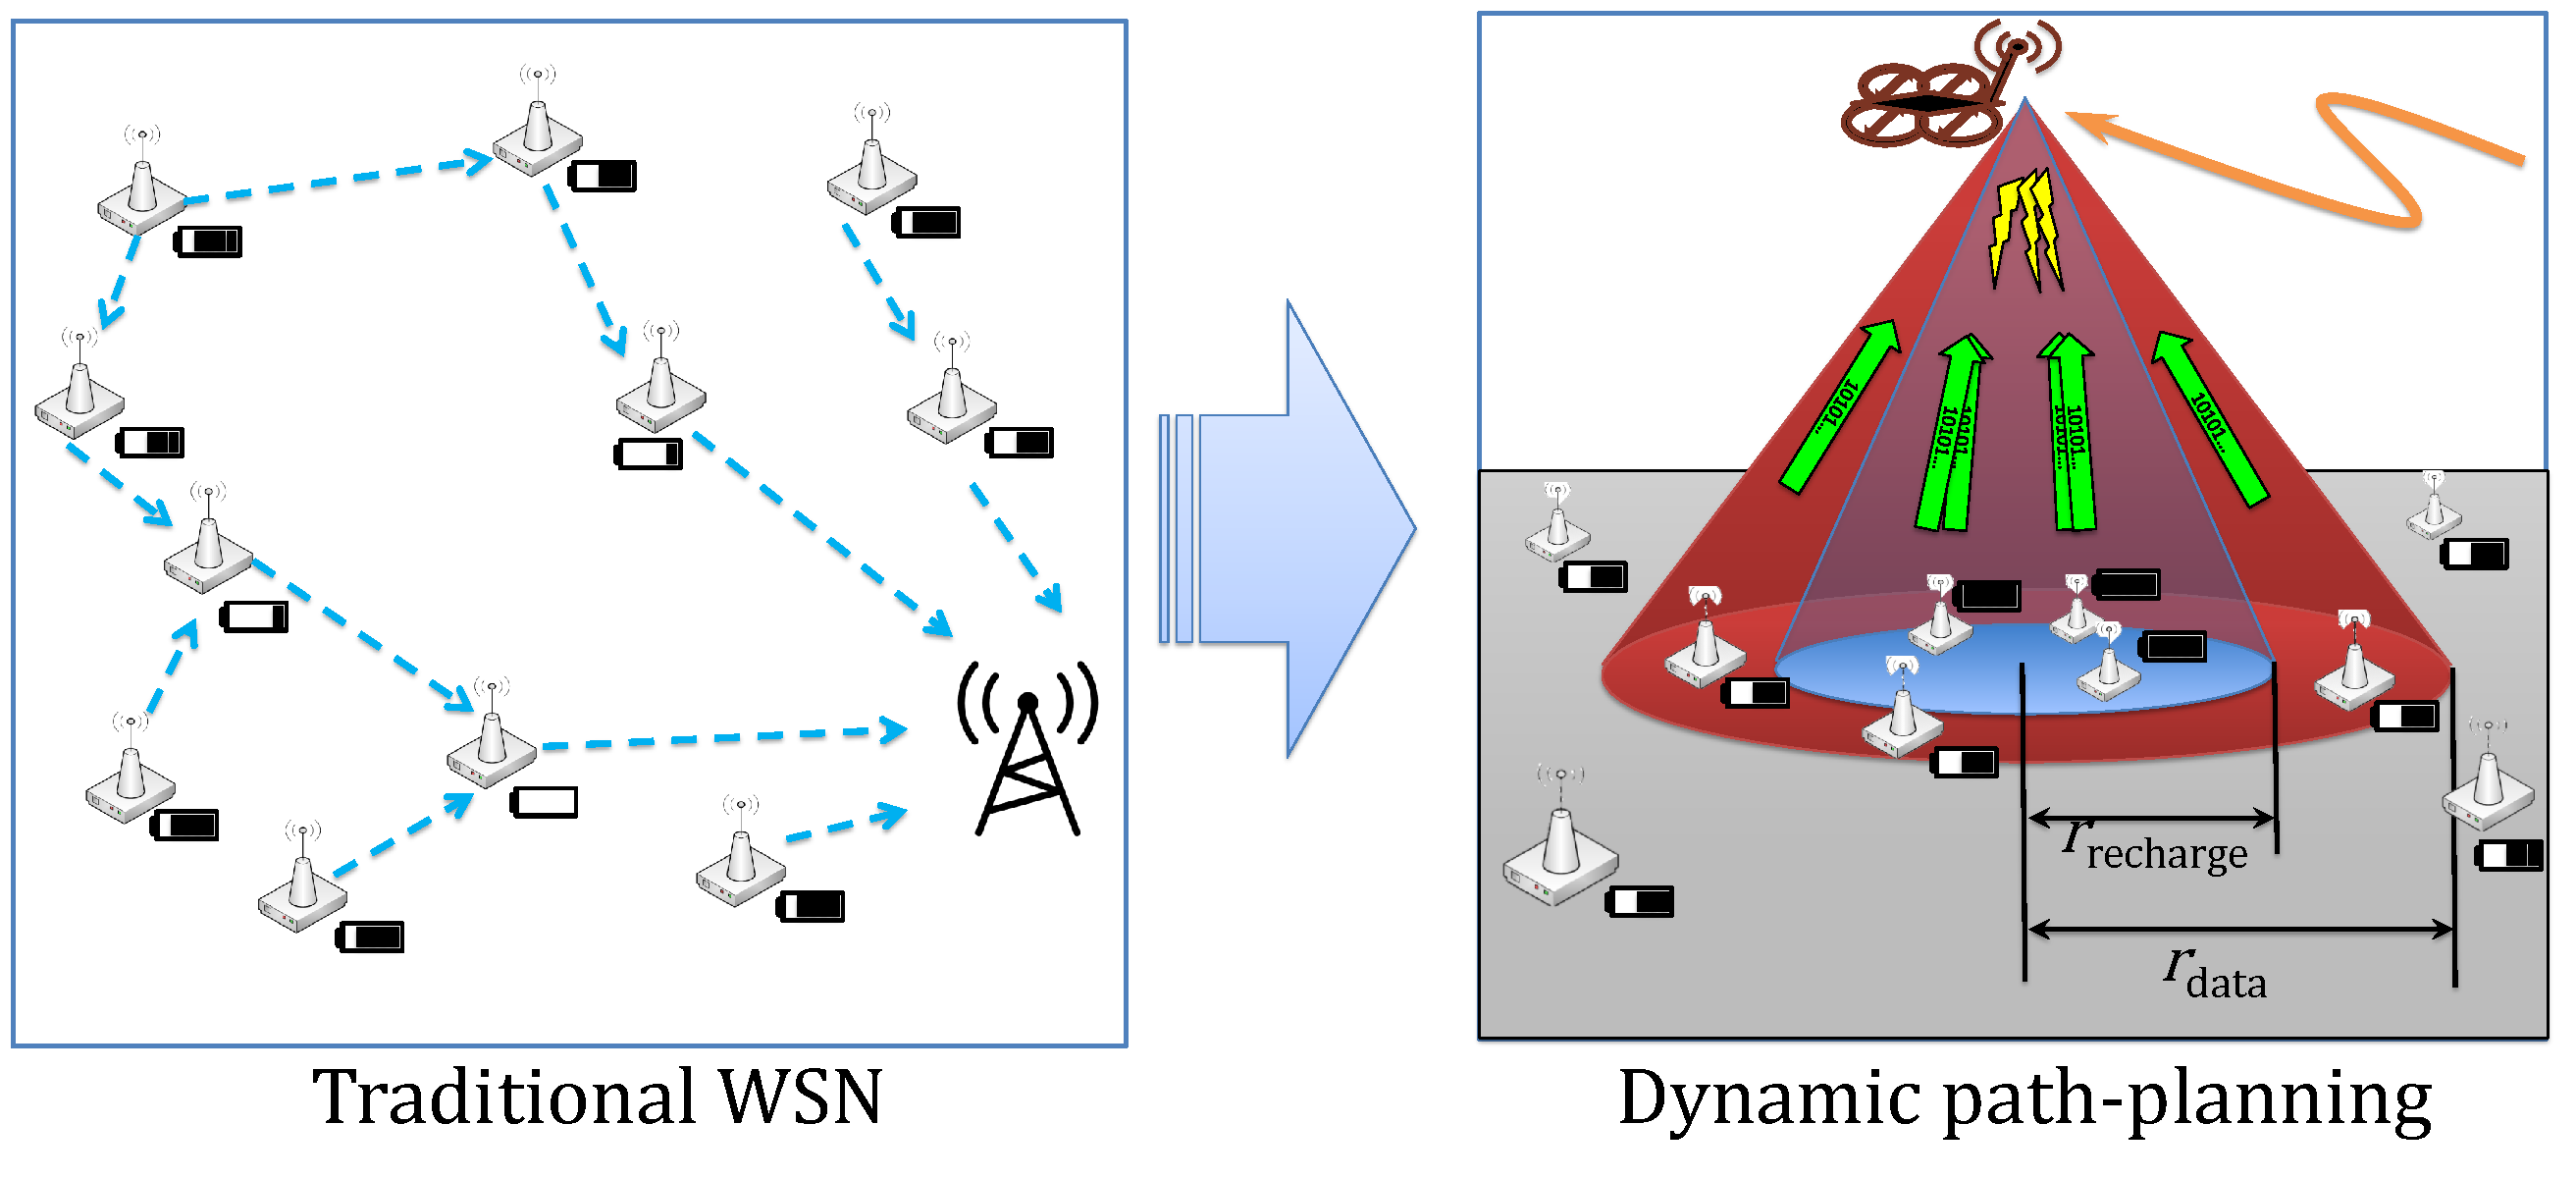
\includegraphics[width=\columnwidth]{overall.pdf}}
 \caption{Evolution from traditional wireless sensor networks (WSNs) to servicing WSN with UV(s). We present path-planning techniques that use unmanned vehicles (UVs) to gather aggregated data and recharge sensors.\label{fig:overall}} 
\end{figure}



\begin{figure} \centering
  {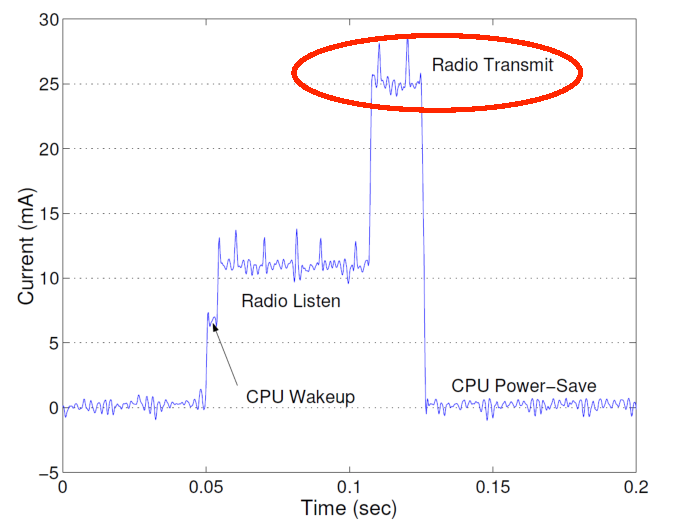
\includegraphics[width=\columnwidth]{txenergy}}
 \caption{Power usage in a wireless sensor node is dominated by transmission costs and listening costs.  Figure modified from~\cite{VsMh04}.} \label{fig:txenergy}
\end{figure}
 
Fortunately, recent breakthroughs in the area of wireless power transfer technologies (e.g. inductive coupling, magnetic resonant, and RF energy harvesting)~\cite{AkAkSE07}  provide promising alternatives for deploying such WSNs. \emph{Magnetic resonant wireless power transfer}~\cite{AkAkSE07} can wirelessly transfer electric power from the energy storage device to the receiving device efficiently within medium range (40\% efficiency within 2 meters). It is also insensitive to the neighboring environment and does not require a line of sight between the charging and receiving devices. Researchers proposed that a mobile unmanned vehicle (UV) carrying a wireless charging device could  visit and recharge each sensor to sustain a WSN~\cite{XySyNT12}.

However, one UV may not be able to visit every sensor if the WSN is deployed in harsh environments/terrains (e.g. dense forest, mountains, underwater), or the WSN is large-scale, consisting of a great number of sensors. Although these seminal studies replenished sensor energy, most of the energy was still wasted by long-distance wireless transmissions of perceived data, especially by relaying sensors. Due to charging and travel time of the UV, some bottleneck sensors may  drain their residual energy while waiting for the UV. Great unsolved challenges on control remain, including how to select the optimal path for the UV to travel within WSNs and how to efficiently dispatch multiple UVs to recharge WSNs.

Assigning sensors to UVs using matching theory often assumes that energy costs due to power transmission greatly exceed the UV's transportation costs.  This assumption might not fit for WSNs spread over large geographic areas, or terrain with obstacles, %% OR not OF
or where transportation costs are high, such as subsea or aerial UVs. This paper focuses on algorithms that make such WSNs sustainable by focusing on path-planing, trajectory optimization, and responding to dynamic network conditions, as shown in Fig.~\ref{fig:overall}.




\section{Related Work}
%I haven't read these papers, and so don't feel comfortable repeating them:
%Energy issues make current WSNs unsustainable. Prior work reduces consumption, but cannot fundamentally resolve the energy issue~\cite{AkSu02,CpSAHCN06,KwfSF08,YpPSN10,FbNbRbICC09}. Wireless power transfer technologies~\cite{AkAkSE07,1AcMdDm14,2JgRcJl13,3CvGd14,38Ns12} add a new dimension to this research. Some pioneering works employ UVs to recharge WSNs to prevent the sensors from depleting their energy~\cite{CwYYangIPDPS2013,xie2013wireless,RenewSN12,XySyNT12,YpPSN10,ZlYp2011}. However, most energy is consumed by long-distance wireless transmissions and there are significant challenges in UV path-planning. Below, we recap wireless power transfer technologies, existing robot-planning solutions, and the applications of each to WSNs.
%
%Wireless power transfer is a technology that enables transmitting energy through vacuum or an air gap to electrical devices without using wire or any other substance. This can be used for a wide variety of applications from low-power toothbrushes, to high-power electric vehicles, where conventional wires are unaffordable, inconvenient, dangerous, expensive or impossible~\cite{60Jg07,61AkkiJh96,63ZcYlKs,64FtKzWy12,65HgHoRm14,66HgMdFb14,67YlYhXl14,93HjJzSs10,94HjJzDl13,95AaSkAa12,96ArGl13,97ArGl12,98ArSmCm11,99RxKcMj13,100QxHwZg13,101QxHwZg13,102GyCd12,103DaSh14}. Wireless power transfer can be generally classified into non-radiative technology~\cite{AkAkSE07,46AkJjMs08,47BcJhDs09,48CzKlCy08,49ZlRcRt09,50JcYrDk12,51DkKkNk12,52AkRmMs10,53KrFk11,54Witri,88HkCsJk14,98ArSmCm11,99RxKcMj13,100QxHwZg13,101QxHwZg13,102GyCd12,103DaSh14,9GcJb13,33ShJwWf13,39XwZwHd14,40CwGcOs04,41ZpSl12,42SaMi08,43LrFaGo13,44HwAgKs12,45JjDk14,81hwAgks12,82MeDoJh07,83NlTh,84UmDj11,85MkMkLt,93HjJzSs10,94HjJzDl13,95AaSkAa12,96ArGl13,97ArGl12} and radiative RF-based technology~\cite{7LxYsTh13,8AsDyPp08,36Zp13,55RzCh13,56Lv08,57KhVl14}. The non-radiative technology, which is based on coupling, consists of inductive coupling~\cite{9GcJb13,33ShJwWf13,39XwZwHd14,40CwGcOs04,41ZpSl12,42SaMi08,43LrFaGo13,44HwAgKs12,45JjDk14,81hwAgks12,82MeDoJh07,83NlTh,84UmDj11,85MkMkLt,93HjJzSs10,94HjJzDl13,95AaSkAa12,96ArGl13,97ArGl12}, magnetic resonant coupling~\cite{AkAkSE07,46AkJjMs08,47BcJhDs09,48CzKlCy08,49ZlRcRt09,50JcYrDk12,51DkKkNk12,52AkRmMs10,53KrFk11,54Witri,88HkCsJk14,98ArSmCm11,99RxKcMj13,100QxHwZg13,101QxHwZg13,102GyCd12,103DaSh14}, and capacitive coupling~\cite{35MkIiBb11,37Sh13}. The radiative RF-based charging can be further sorted into directive RF and non-directive RF power transfer~\cite{36Zp13}. Magnetic \emph{inductive} coupling uses a magnetic field to deliver electrical energy between two coils. Due to low quality factors, the effective charging distance is generally within 20cm. Magnetic \emph{resonant} coupling is based on evanescent wave coupling to generate and transfer electrical energy between two resonant coils through varying or oscillating magnetic fields. Magnetic resonant coupling can transfer power over longer distance than inductive coupling, and its efficiency is better than an RF radiation approach. In 2007, MIT scientists demonstrated that magnetic resonant coupling can light a 60W bulb more than two meters distant with an efficiency around 40\%~\cite{AkAkSE07}. Inductive coupling and resonance coupling have been widely used in many fields including: robot manipulation, automated underwater vehicles, induction generators, induction motors, and biomedical implants~\cite{60Jg07,61AkkiJh96,63ZcYlKs,64FtKzWy12,65HgHoRm14,66HgMdFb14,67YlYhXl14,93HjJzSs10,94HjJzDl13,95AaSkAa12,96ArGl13,97ArGl12,98ArSmCm11,99RxKcMj13,100QxHwZg13,101QxHwZg13,102GyCd12,103DaSh14}. RF radiation utilizes diffused RF/microwave as a medium to carry radiant energy. It can also use other electromagnetic waves such as infrared and X-rays. However, due to safety issues raised by RF exposure, these bands are not widely used.  RF/microwave energy can be radiated isotropically or toward some direction through beamforming. RF/microwave radiation is generally used for far-field charging. Applications vary, including TV broadcast, AM radio broadcast and GSM bands (900/1800), as well as WiFi routers, cellular base stations, and satellites~\cite{137PnMnKc13,138XwAm13,139LbNbHs14,140TlNlBp13,141EkAhMb14,142FaMaSa14,143ApAsYz13,144AtHaLd13}.

%Relevant literature from robotics:
The path-planning problem for UVs has been investigated from several angles. To minimize path length, the authors in~\cite{bektas2006multiple}  survey the multiple-Traveling Salesman Problem, itself a generalization of the vehicle routing problem~\cite{dantzig1959truckdispatchingproblem}. Servicing a WSN is closely related to coverage problems, recent work includes methods for optimizing speed along given routes~\cite{smith2012persistent}, and techniques to continually improve existing routes~\cite{soltero2013decentralized}. 
Much work has focused on the data ferrying problem, from minimizing the latency between visits to nodes~\cite{Alamdari:2014:PMD:2568343.2568350}, to maximizing the total data rate from sensors to sink using UVs \cite{huang2014resource}, to minimizing overall delay  while sharing bandwidth~\cite{Guo:2007:FES:1364654.1364671}, to having a set schedule and opportunistically deviating from it \cite{guo2006opportunistic}.

Using unmanned aerial vehicles to recharge other robots or sensor nodes has focused on physical design, which includes direct contact, such as swapping batteries~\cite{toksoz2011automated,swieringa2010autonomous} or direct recharge~\cite{mulgaonkar2012automated}, wireless resonant coupling~\cite{griffin2012resonant,johnson2013charge,jung2012inductive}, and electromagnetic radiation~\cite{xie2013wireless}, and algorithmic improvements using graph theory~\cite{mathew2013graph}, linear programming~\cite{smith2012persistent}, and gradient descent optimization~\cite{soltero2013decentralized}. 

Finally, data aggregation and recharging shares similarities with persistent robotic tasks, such as cleaning, mowing, observing, and patrolling\cite{mackenzie1996making,kakalis2008robotic,Choset2001,Cortes2004,smith2012persistent,arkin2000approximation,correll2009building,soltero2013decentralized}


\section{ Overview}
This paper's goal is to explore path-optimization techniques. 
Previous work often uses optimization/matching theory to assign one UV/multiple UVs to WSN nodes, and use a Hamiltonian cycle to visit each node.  This is reasonable if recharging nodes is the largest component of a UV's energy budget: $ E_{\rm{recharge}} |\rm{nodes}| \gg E_{\rm{movement}} *
\rm{path\_length}$.  If this assumption is violated, path-planning becomes the key concern.  A simplified form of this decision is written as  
\begin{equation}
K_{dist} = \frac{E_{\rm{movement}} *
\rm{path\_length}}{E_{\rm{recharge}} |\rm{nodes}|}.
\label{eq:TippingPointDistance}
\end{equation}
 Here $K_{dist}$ represents the \emph{tipping point}, the variable where the decision problem becomes fundamentally different.  If $K_{dist}$ is small, path-planning is inconsequential, and almost any solver is sufficient.  However, when $K_{dist}$ is large path-planning becomes the key consideration. Our eventual goal is to design full trajectories that optimize the path of each UV, by servicing multiple nodes simultaneously.  However, even just  the path-planning component is NP-hard~\cite{arkin2000approximation}. To make progress, this paper focuses on path optimization techniques. 

%A key tipping point in these problems is if a UV can service multiple clients simultaneously.  

A UV has an associated recharging footprint and a data-transfer footprint, which can often be modeled as disks of radius $r_{recharge}$ and $r_{data}$, as illustrated in Fig.~\ref{fig:loadDensity}. If sensor nodes are clustered, a UV can service multiple clients simultaneously.  

\begin{figure} \centering
  {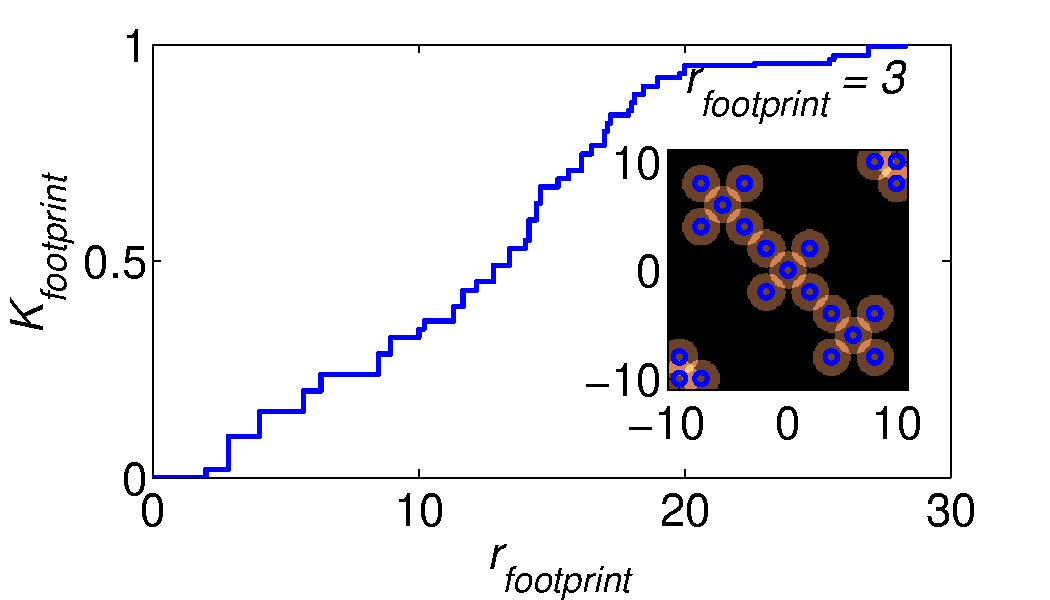
\includegraphics[width=\columnwidth]{Kfootprint}}
 \caption{ As the recharging footprint or data-transfer footprint $r_{footprint}$ grows, more sensors can be recharged simultaneously. The plot above shows $K_{footprint}(r_{footprint})$, and given by \eqref{eq:Kfootprint}.
 \label{fig:footprint}}
\end{figure}

We represent the fraction of sensors that are clustered as 
\begin{equation}
K_{footprint} = \frac{2}{N^2-N}  \sum_{i=1}^N \sum_{j=i+1}^N \left(  \left\| p_i - p_j \right\| _2  \le r_{footprint} \right). \label{eq:Kfootprint}
\end{equation}
%$K_{footprint} = \frac{1}{N}  \sum_{i=1}^N (\underset{j\mei, j\in [1,N]}{\text{minimize}} ||p_i - p_j ||_2 ) \le r_{footprint}$. 
%$K_{footprint} = \sum_{j=i+1}^N  \sum_{i=1}^N ||p_i - p_j ||_2  \le r_{footprint}$. 
Here, $p_i$ is the position of the $i$th node, and there are $N$ nodes. $K_{footprint}$ is shown in  Fig.~\ref{fig:footprint} for a representative network.

 In general, energy-efficient recharging requires closer proximity than data transmission, so this implies there are two tipping points related to node density, $K_{recharge}$, and $K_{data}$.   
 Correspondingly, the WSN recharge problem has three regimes with differing solutions. 
 Before the tipping points, nodes are sparse and not clustered.  In this regime optimal paths are straight lines from node to node, and the optimal solution is a variant of the traveling salesman problem.  As sensors get closer together, the optimal path may be \emph{between} one or more sensors.   In Fig.~\ref{fig:loadDensity}, path \textbf{A} is designed to visit each node, but path \textbf{B} is designed to recharge all nodes.  Here, the optimal solution is often to weave between clusters of nodes.  The third regime is when many nodes are close enough for transfer data, as shown in path \textbf{C}.  The simulations in this paper take advantage of the non-zero $r_{footprint}$ to allow the UVs to pass near sensors without requiring them to visit each node.
 
 \begin{figure}
\begin{overpic}[width =\columnwidth]{loadDensity}\end{overpic}
\centering \vspace*{-.1in}
\caption{\label{fig:loadDensity}
A UV has an associated recharging footprint and a data-transfer footprint, which can often be modeled as disks of radius $r_{recharge}$ and $r_{data}$.  
Path \textbf{A} visits each node, but path \textbf{B} is shorter because it is designed merely to recharge all nodes.  Path \textbf{C} is the least tortuous because it is designed to transfer data from all nodes, and $r_{data}>r_{recharge}$. %We will design speed controllers to service multiple clients when sensors are dense or clustered.
} \vspace*{-.1in}
\end{figure}
 
%Our eventual goal is to design full trajectories that optimize the path of each UV, by servicing multiple nodes simultaneously.  However, even just  the path-planning component is NP-hard~\cite{arkin2000approximation}. To make progress, we decouple the problem and optimize the \emph{speed} of UVs along prescribed paths to service multiple clients when sensors are dense or clustered. This approach is reasonable for ground-based mobile UVs that are constrained to roads or trails, and aerial UVs constrained to air corridors.
%%The mobile robotics community has investigated optimal path-planning for similar problem, such as harvesting agricultural products~\cite{correll2009building}, recovering oil from a spill \cite{kakalis2008robotic}, cleaning dirt from a room~\cite{mackenzie1996making}, and recharging WSNs~ \cite{Cortes2004}.
%We will augment existing solvers~\cite{smith2012persistent} to account for battery levels of the nodes and UV.  We will pose this as an LP, and share code on Matlab central. Solutions will be compared to results using matching algorithms in task 2.
%


%\begin{wrapfigure}{r}{0.4\textwidth}
%  \vspace{-20pt}
%  \begin{center}
%  \includegraphics[width=0.4\textwidth]{hgridsrand50.eps}
%  \end{center}
%  \vspace{-20pt}
%%  \caption{Revenue upper bounds: $|\mathcal{H}|$ = 2, 3 and 4.}\label{fig:RevenueDiffBandRGT}
%  \caption{Performance of different algorithms.}\label{Fig:simu}
%  \vspace{-7pt}
%\end{wrapfigure}


%\subsubsection{Hardware implementations}\label{subsubsec:quadcopterTestbed}
%Hardware implementations generate confidence in solutions, often uncover assumptions in our theory, and are excellent for teaching.  Our initial implementations will use an existing fleet of eight medium-scale mobile robot bases (ERA). These robots are ideal for demonstrating WSN servicing because  they are simple, have a long battery life, and  are highly expandable. Each robot fits within a 40cm cube, and can be accurately tracked with our OptiTrack motion capture system, allowing us to quickly focus on the algorithms.  


\section{Path Optimization Algorithm}\label{sec:algorithm}
Our solution designs a closed-loop path that intersects the origin for each UV.   The base technique is a variant of Lloyd's algorithm~\cite{lloyd1982least,Becker2013l}. Each path is represented by a finite number of waypoints, and these waypoints are both attracted to the centroid of all sensor nodes within their Voronoi cell, and attracted to their neighboring waypoints.  The following sections describe how this path is initialized (\ref{subsec:InitializingPath}), and then how the path is optimized by switching between a gradient descent optimization routine that finds local minimas (\ref{subsec:gradientDescent}), and a genetic algorithm that rearranges the order of waypoints to improve the paths (\ref{subsec:TSP}). Our {\sc Matlab} implementation is available at \href{http://www.mathworks.com/matlabcentral/fileexchange/49863-decentralizedpathplanningforcoverageusinggradientdescent}{mathworks.com/matlabcentral/fileexchange/49863}~\cite{Srikanth2015}. 




\subsection{ Initializing Path with Hilbert Curve}\label{subsec:InitializingPath}
It is important to have an initial path that fills the map. This ensures the UVs will visit  every node. We adapt the space-filling \emph{Hilbert Curve}, which creates a fractal path that fills up a unit area space and serves as an initial path for the first iteration~\cite{fischer1928darstellung}. Figure~\ref{fig:OneUAVsim} shows an initial path using a Hilbert curve.  If there are multiple UVs, the Hilbert curve is scaled by a scalar to ensure the waypoints are unique, as shown in Fig.~\ref{fig:multipleUAVsim}.

\subsection{ Gradient Descent on a Path Composed of Waypoints}\label{subsec:gradientDescent}
The following algorithm is derived from \cite{soltero2013decentralized}, which focused on local optimization techniques that gradually improve the paths followed by robots during persistent tasks. This technique is amenable to WSN. 

Consider $N$ UVs servicing a Wireless Sensor Network in a convex, bounded area $\mathbf{Q}\subset{ \mathbb{R}^2}$.
Waypoints are a set of points that define the path for each UV. The UV travels in a straight line in between two neighboring waypoints.
Let $\mathbf{p}_i^r$ be the position of the $i^{th}$, $i\in(1\ldots n(r))$ waypoint of the $r^{th}$ UV. Servicing includes recharging the nodes and collecting a part of the data that the nodes are about to transmit to the sink there by reducing the power expenditure in the sensor nodes. The algorithm forms a locally-optimal path to visit the sensor nodes in the WSN.  At each step, we compute the Voronoi partition $\mathbf{V}_i^r$ defined by the waypoints, with one partition assigned to each waypoint.

 We require a function  $\phi(\mathbf{q})$ that designates how many sensor nodes can be recharged at the position $\mathbf{q}$.
%commands the usefulness of a location on the map for servicing the WSN (${\mathbf{q}\in{Q}|\phi(\mathbf{q})>0}$) .
This function is used to define a cost function for each path:
\begin{align}\label{eq:cost-function}
\mathbf{H} = \sum\limits_{r=1}^N\sum\limits_{i=1}^{n(r)} \int_{V_i^r}\frac{\mathbf{W}_s}{2}\|q-p_i^r\|^2&\phi(\mathbf{q}) d\mathbf{q}&+\nonumber\\
\sum\limits_{r=1}^N\sum\limits_{i=1}^{n(r)}\frac{\mathbf{W}_n}{2}\|p_i^r-p_{i+1}^r\|^2
\end{align}

$\mathbf{W}_s,\mathbf{W}_n$ are positive scalar constants that are used to weight the sensing and neighbor distance, respectively, and depend on the experimental setup.
The gradient descent algorithm minimizes the two-part cost function \eqref{eq:cost-function}. The first part of the equation indicates waypoints in regions far away from sensor nodes is costly and the second part indicates having neighboring waypoints far away is also costly. A minimizing solution is a short path that mostly travels near WSNs. 


We compute the mass, mass-moment, and centroid of the $V_i^r$ (Voronoi partition for $\mathbf{i}^{th}$ waypoint of the $\mathbf{r}^{th}$ UV ) as follows:
\begin{align}\label{eq:massmomentcentroid}
M_i^r &=  \int_{V_i^r}\phi(\mathbf{q}) d\mathbf{q}, \quad
\mathbf{L}_i^r =  \int_{V_i^r}\mathbf{q}\phi(\mathbf{q}) d\mathbf{q}, \nonumber\\
\mathbf{C}_i^r  &= \frac{ \mathbf{L}_i^r } { M_i^r  }
\end{align}

The control law for each waypoint is the summation of forces that pulls the waypoint toward the centroid of the Voronoi partition (weighted by $\phi(\mathbf{q})$)
\begin{align}\label{eq:controllaw}
\mathbf{u}_i^r  = \frac{ K_i^r (M_i^r \mathbf{e}_i^r + \boldsymbol{\alpha}_i^r)} { \beta_i^r  }
\end{align}
Here, $\mathbf{K}_i^r$ is a positive definite matrix and is potentially-time varying. $\mathbf{e}_i^r = \mathbf{C}_i^r  - \mathbf{p}_i^r$, the error, introduces the first primitive by obtaining the difference between the waypoint position and the weighted centroid of the Voronoi region. This tries to move the waypoint towards the interesting region, reshaping the path of the robot. The second term  
$ \boldsymbol{\alpha}_i^r = W_n( \mathbf{p}_{i+1}^r  + \mathbf{p}_{i-1}^r -2 \mathbf{p}_{i}^r)$ introduces the second primitive which pulls the neighboring waypoints together to obtain a short path. $\boldsymbol{\beta}_i^r = \mathbf{M}_{i}^r + 2\mathbf{W}_{n}$ normalizes the weight distribution between servicing sensors and staying close to neighboring waypoints.


The control is then applied to each waypoint and update their positions:
\begin{align}\label{eq:state evolution}
\mathbf{p}_i^r(k)  = \mathbf{p}_i^r(k-1) + \mathbf{u}_i^r 
\end{align}
The control algorithm is described in Alg. \ref{alg:ICpathcontrol}.

\begin{algorithm}
\caption{Gradient descent path optimization for the $i^{th}$ waypoint $\mathbf{p}_i^r$ in robot $r$'s path in a known environment (from~\cite{smith2012persistent}, implemented at \cite{Srikanth2015}).
\label{alg:ICpathcontrol}}
%Algorithm: IC (Interesting Closed) path controller for the $i^{th}$ waypoint $p_i^r$ in robot $r$�s path in a known environment. (from~\cite{smith2012persistent}) \\
\begin{algorithmic}[1]
\Require Ability to calculate Voronoi partition 
\Require Knowledge of the location of neighboring waypoints  $\mathbf{p}_{i-1}^r $ and $ \mathbf{p}_{i+1}^r$
\Loop
\State  Compute the waypoint�s Voronoi partition 
\State  Compute $\mathbf{C}_i$ according to \eqref{eq:massmomentcentroid}
\State  Obtain neighbor waypoint locations $\mathbf{p}_{i-1}^r$  and $\mathbf{p}_{i+1}^r$
\State  Compute $\mathbf{u}_i^r$  according to \eqref{eq:controllaw}
\State  Update $\mathbf{p}_i^r$  according to \eqref{eq:state evolution}
\EndLoop
\end{algorithmic}
\end{algorithm}




\subsection{ multiple-Traveling Salesman Problem (mTSP)}\label{subsec:TSP}
The gradient descent algorithm  (Alg. \ref{alg:ICpathcontrol}) can get stuck in local minima.  To further improve the path we input the location of the waypoints obtained after running the gradient descent algorithm into a multiple-Traveling Salesman Problem (mTSP) search algorithm. 
Given a list of cities to visit, the classic \emph{traveling salesman problem} (TSP) attempts to find an ordering of the cities that minimizes the total distance on a tour that visits all the cities once\cite{applegate1999finding}.  The solution is the shortest Hamilton cycle. By labelling our sensor nodes as cities, the solution to the traveling salesman problem gives the shortest length path. The mTSP solution straightens out loops in the path and can reduce the cost function.  This often moves the solution out of the local minimum obtained after the executing the gradient descent algorithm. 


  This problem is NP-hard (Non-Deterministic Polynomial), but many powerful heuristics are available, and software packages can provide answers for tens of thousands of nodes (e.g., the Concorde TSP Solver~\cite{applegate2002minmax}).
A solution with multiple salesman is called a mTSP.  The mTSP is still an NP-hard  problem~\cite{arkin2000approximation}, so the solutions returned by the search algorithm given limited time may not be the global optimum. 

 A good heuristic can increase TSP solver performance.   In our  numerical simulations, priming an open-source genetic algorithm solver\cite{Kirk2014} by sorting the nodes by angle from the sink and dividing the sorted list equally between the UVs decreased path costs by 20\%.  Figure \ref{fig:mTSPsim} shows results from our simulation with 100 nodes and 5 UVs.



\begin{figure}\centering 
\newcommand{\figheight}{1.4in}
\subfigure[nodes partitioned by angle\label{subfig:tspCities}]
  {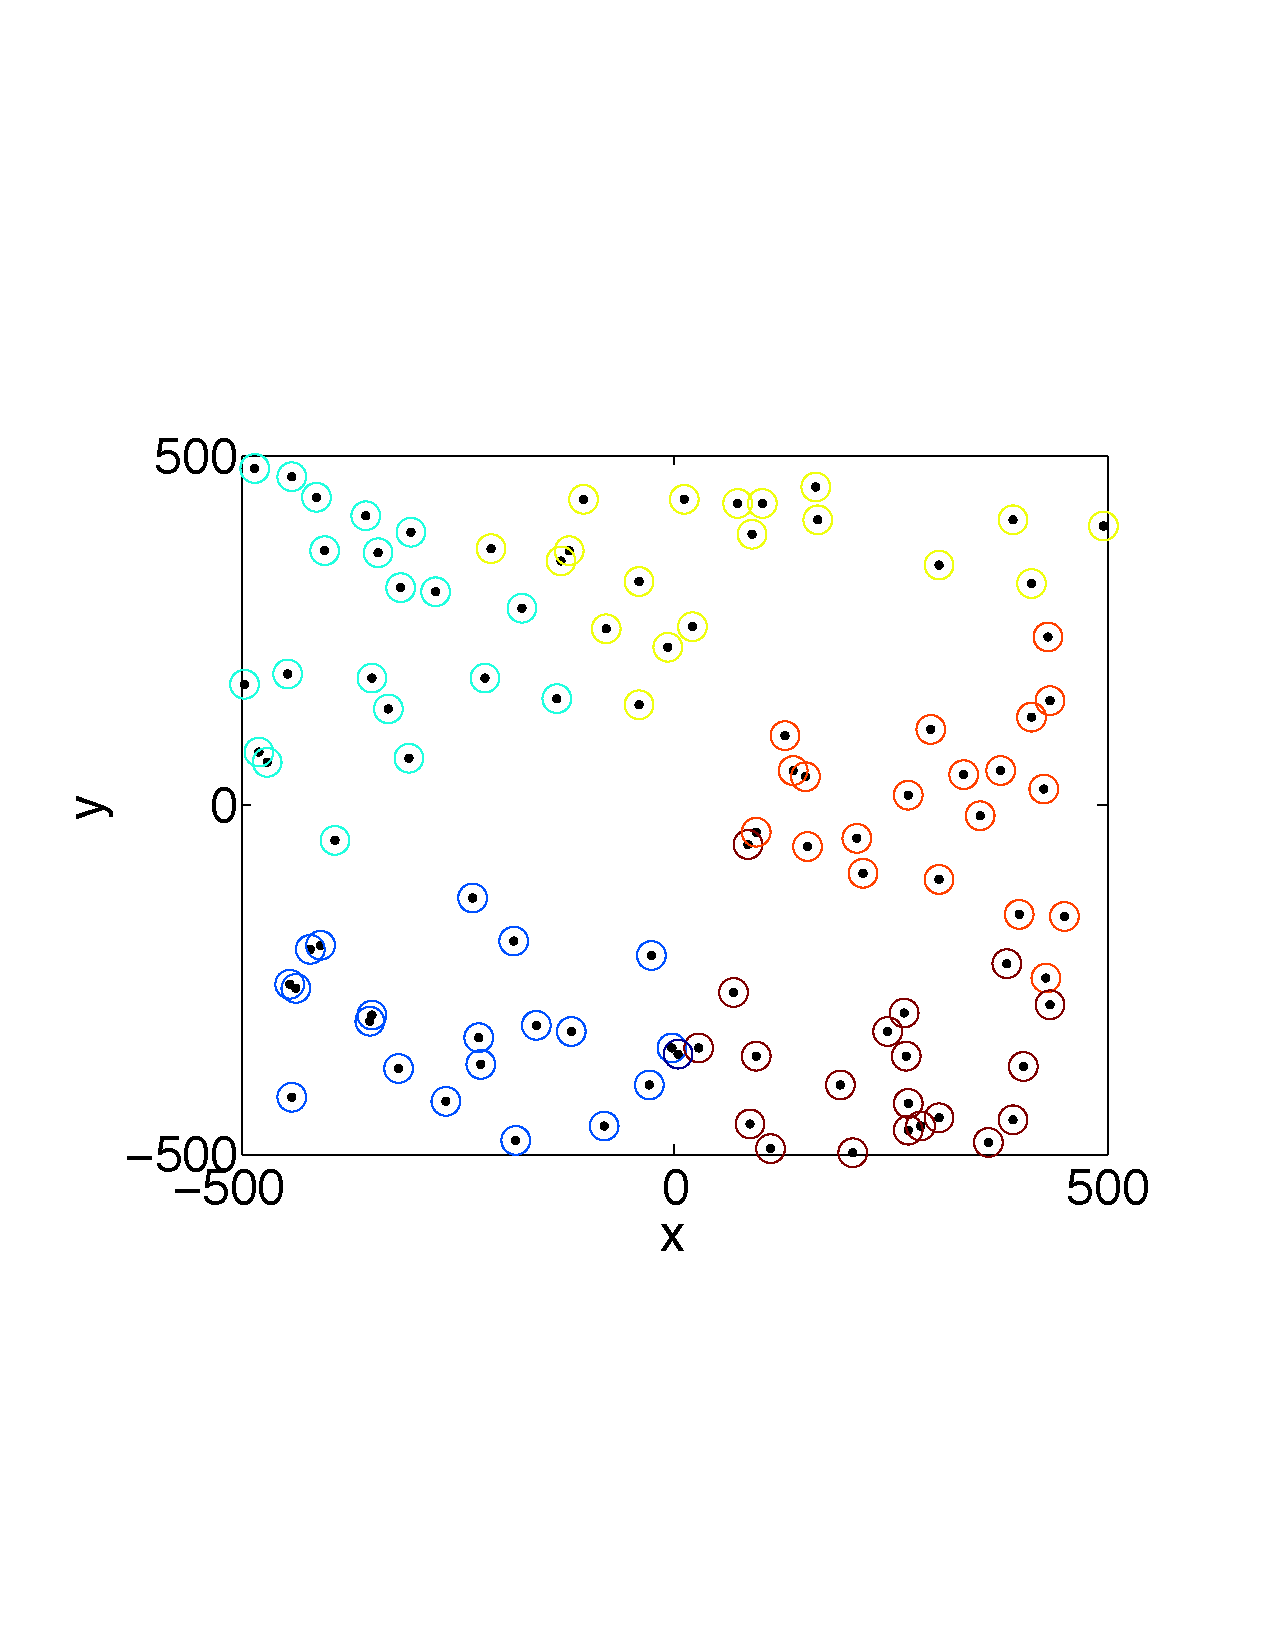
\includegraphics[width=.45\columnwidth]{tspCities.pdf}}
 \subfigure[near-optimal solution.\label{subfig:tspPaths}]
  {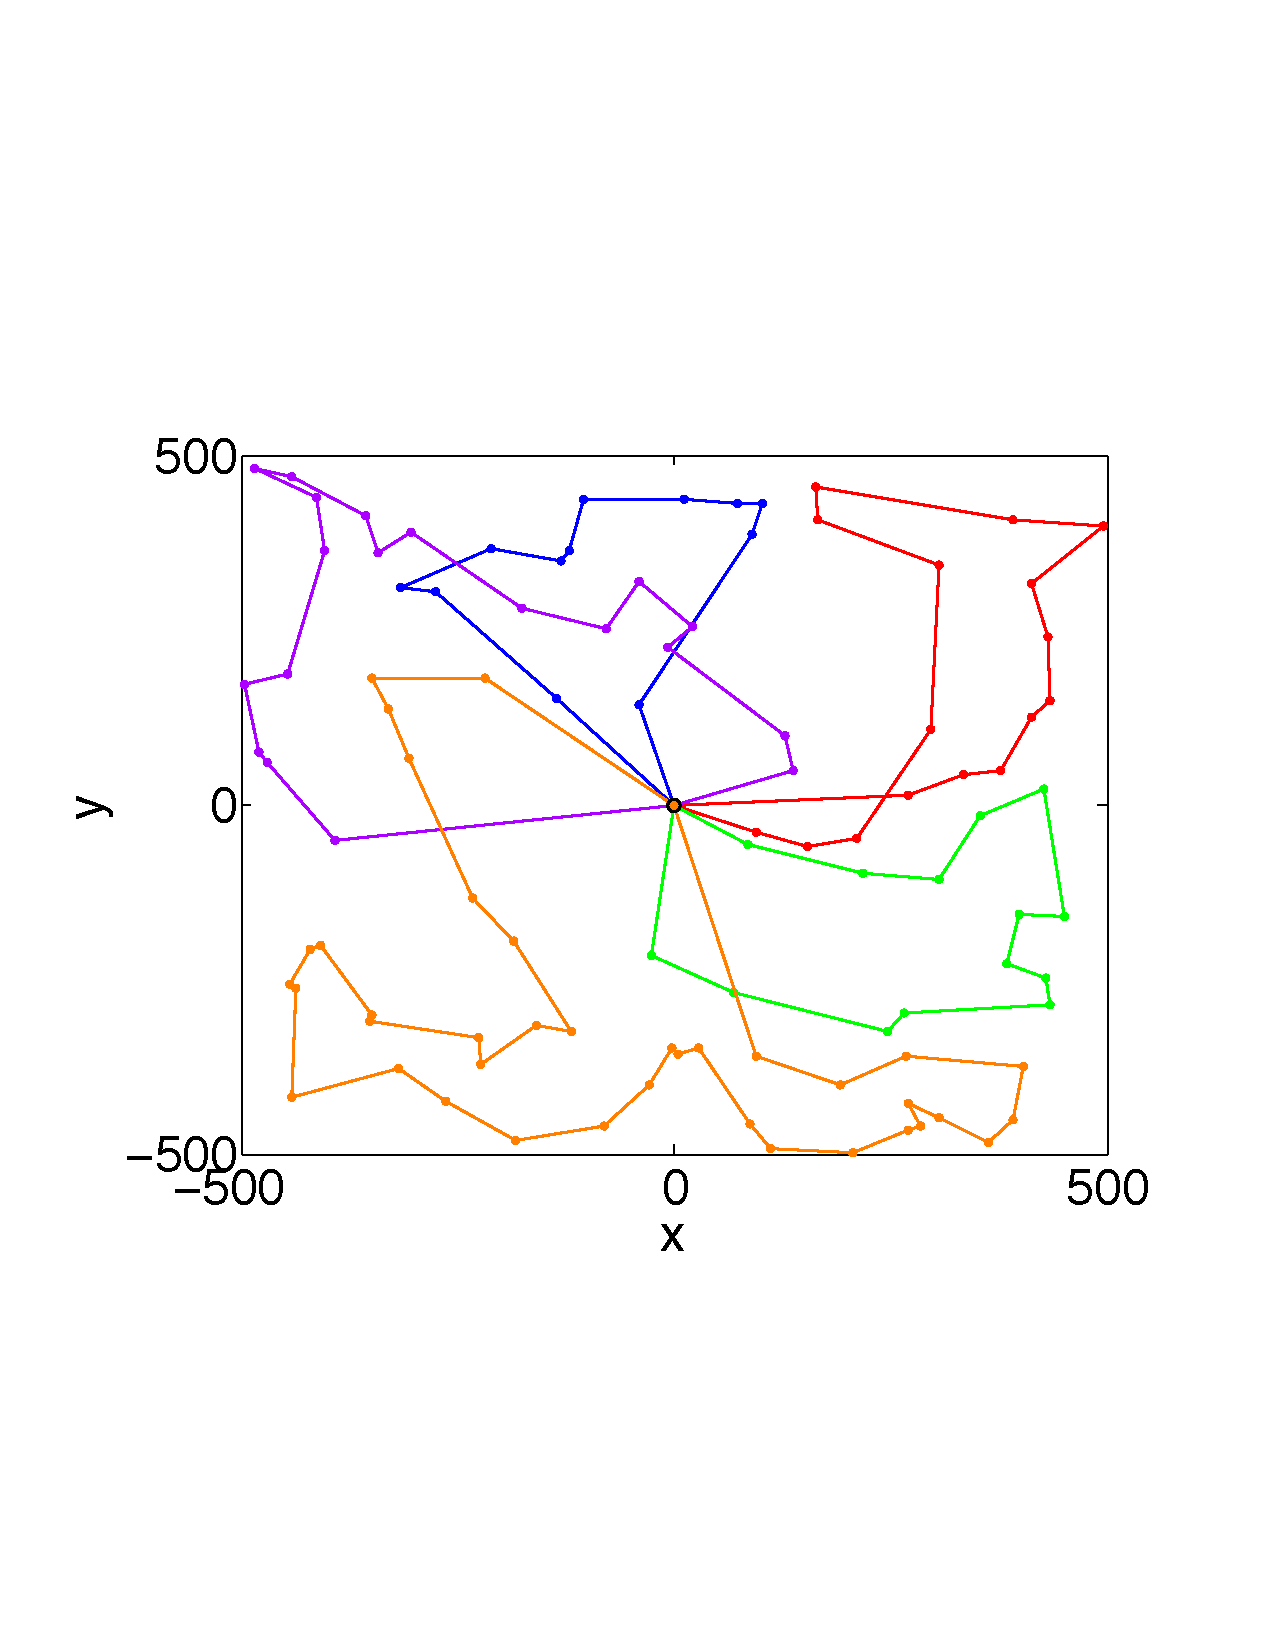
\includegraphics[width=.45\columnwidth]{tspPaths.pdf}}
   \vspace*{-.1in}
 \caption{Screenshots from mTSP solver aided by heuristic.  Left, nodes partitioned according to angle from sink. Right, near-optimal solution from a mTSP solver aided by our heuristic.   \label{fig:mTSPsim}}
 \vspace*{-.1in}
\end{figure}

%%\begin{wrapfigure}{r}{0.6\textwidth}
%\begin{figure}
%\begin{overpic}[width =0.33\columnwidth]{tspCities.pdf}\end{overpic}
%\begin{overpic}[width =0.33\columnwidth]{tspPaths.pdf}\end{overpic}
%\begin{overpic}[width =0.33\columnwidth]{Task3Experiment}\end{overpic}
%\caption{\label{fig:mTSPsim}
%Left and center: screenshots from mTSP solver aided by heuristic.  Left, nodes partitioned according to angle from sink. Center, near-optimal solution. Right, preliminary hardware experiment design.  Using our motion tracking system, we can abstract the problem of localizing our sensor nodes and focus on implementing  path-planning algorithms.
%}
%\end{figure}


\section{Results}

We developed a {\sc Matlab} simulation using the three algorithms described in Section \ref{sec:algorithm}.  The code is available at \cite{Srikanth2015}. The next two sections describe the results with one UV and with multiple UVs.

\begin{figure*}
\centering
\renewcommand{\figwid}{0.4\columnwidth}
\begin{overpic}[width =\figwid]{1_1}
\end{overpic}
\begin{overpic}[width =\figwid]{1_2}
\end{overpic}
\begin{overpic}[width =\figwid]{1_3}
\end{overpic}
\begin{overpic}[width =\figwid]{1_4}
\end{overpic}
\begin{overpic}[width =\figwid]{1_5}
\end{overpic}
\vspace{-1em}
\caption{Simulation results of optimization algorithm in Section \ref{sec:algorithm} for one UV. 
1.) Iteration 0: Hilbert's Space Filling Curve.
2.) Iteration 100: gradient descent algorithm (first).
3.) Iteration 200: mTSP solver (first).
4.) Iteration 300: gradient descent algorithm (second).
5.) Iteration 400: mTSP solver (second). 
The waypoints are indicated by a set of linked $\circ$ markers, the associated Voronoi diagram is in blue, the magenta lines represent the path the UV follows for servicing the sensor nodes, and the underlying density plot represents the interesting regions generated by the sensor nodes.
\label{fig:OneUAVsim}}
\end{figure*}
\begin{figure*}
\centering
\renewcommand{\figwid}{0.4\columnwidth}
\begin{overpic}[width =\figwid]{2_1}
\end{overpic}
\begin{overpic}[width =\figwid]{2_2}
\end{overpic}
\begin{overpic}[width =\figwid]{2_3}
\end{overpic}
\begin{overpic}[width =\figwid]{2_4}
\end{overpic}
\begin{overpic}[width =\figwid]{2_5}
\end{overpic}
\vspace{-1em}
\caption{
Simulation results of optimization algorithm in Section \ref{sec:algorithm} for two UVs. 
1.) Iteration 0: Hilbert's Space Filling Curve.
2.) Iteration 100: gradient descent algorithm (first).
3.) Iteration 200: mTSP solver (first).
4.) Iteration 300: gradient descent algorithm (second).
5.) Iteration 400: mTSP solver (second). 
The waypoints are indicated by a sets of linked red and yellow$\circ$ markers, the associated Voronoi diagram is in blue, the white and cyan lines represent the path the UVs follow for servicing the sensor nodes, and the underlying density plot represents the interesting regions generated by the sensor nodes.
\label{fig:multipleUAVsim}}
\end{figure*}

\subsection{One UV}
A single UV system was simulated using {\sc Matlab} in Fig.~\ref{fig:OneUAVsim}. The initial path at iteration $0$ was set to be a space-filling Hilbert's curve, to identify the location of the sensor nodes. If the UV follows this initial path it can learn the value function $\phi(\mathbf{q})$, and identifying the interesting points for the whole map. A waypoint at $[0,0]$ is stationary, this represents the sink where the UV recharges and unloads data collected while servicing the sensor nodes. For the first $100$ iterations the gradient descent algorithm moves the path waypoints, using the Voronoi diagram to identify locations with high sensory information. The path achieved after $100$ iterations is usually a local-optimum and iterating further does not decrease the cost function. This sub-optimal solution obtained often contains loops.  To further optimize our path  and escape this local-optimum the path is inputted into a mTSP (multiple-Traveling Salesman Problem) solver for the next $100$ iterations, this straightens the loops by reconnecting the waypoints without changing the waypoint location ($\mathbf{p}_{i}^r$ ). After 200 iterations the cost function has decreased due to straightening of the loops by the mTSP solver. These two algorithms are called in succession to optimize the cost function depending on the time available for calculation or until the cost function asymptotically converges. The cost function is shown in Fig.~\label{subfig:CostFunc1robot}.  This cost function monotonically decreases.  

\begin{figure}\centering 
\newcommand{\figheight}{1.4in}
\subfigure[Cost-function plotted for the single robot case.\label{subfig:CostFunc1robot}]
  {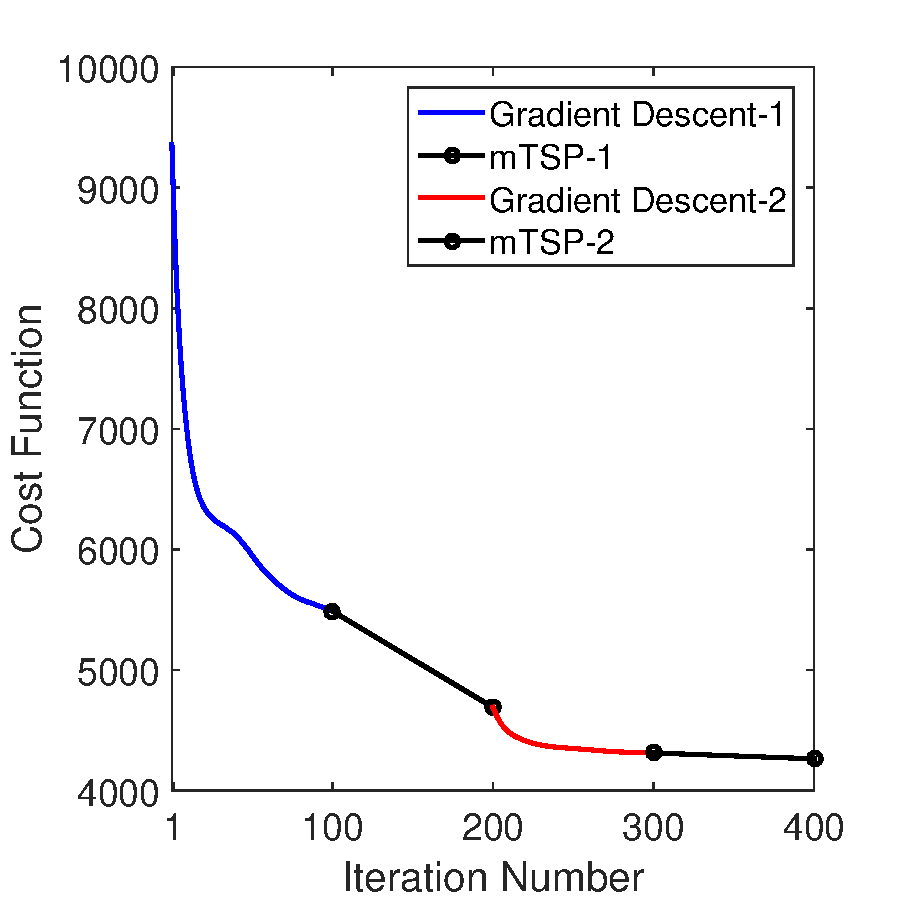
\includegraphics[width=.45\columnwidth]{1_6}}
 \subfigure[Cost-function plotted for the two robot case.\label{subfig:CostFunc2robots}]
  {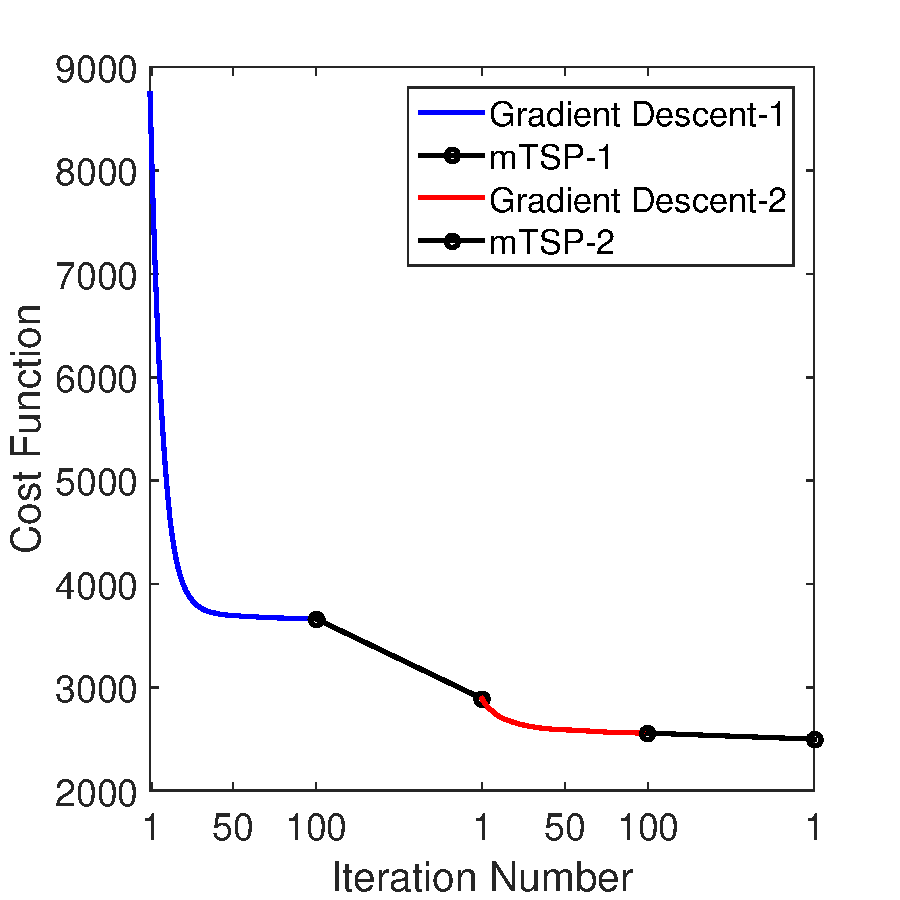
\includegraphics[width=.45\columnwidth]{2_7}}
   \vspace*{-.1in}
 \caption{Cost function indicates a decreasing trend approving the optimization algorithm.\label{fig:CostFunctionSim}}
 \vspace*{-.1in}
\end{figure}

\subsection{Multiple UVs}
A two UV system was simulated on MATLAB. As shown in Fig.~\ref{fig:multipleUAVsim}, UVs service different sets of nodes in the WSN. A multi-UV system is practical  because a single UV might not be able to handle a large network. Similar to the one UV case, a space-filling Hilbert's curve is used to initialize the paths. Each path contains a stationary waypoint at $[0,0]$, representing the sink where both UVs recharge and unload data collected while servicing the sensor nodes. The sensor nodes were placed in random locations to verify the robustness of the algorithm. The algorithm proceeds in a similar fashion to the one UV case. The simulation results show the optimization of the path and the minimization of the cost function.

\section{Conclusion}
An optimized path-planning algorithm was simulated for servicing a WSN. The path constructed is adaptive to the sensor node locations. 
The simulations above used a static WSN, but often sensor data transmission is  dependent on transient phenomena.  For example,  a swarm of subsea sensors may track a school of fish, the progress of an oil slick, or seasonal drift of ocean currents.  These are time-varying phenomena, and so the UV servicing the sensors should be able to adapt.

The same local optimization techniques can iteratively adapt the paths of UVs.  A schematic of our the adaptive control law is shown in Fig.~\ref{fig:dynamicVsStatic}.  
 %We will use both battery levels and the cost of transmitting data to weight the sensor nodes. We will also compare improvements using Newton's method~\cite{seiler1989numerical}. 
Future work should extend our simulation to handle non-stationary sensor nodes, improve the convergence rate, and use our mTSP code to escape local minimal. We are in the process of implementing the algorithm on mobile-robots, with eventual implementation with a set of quadcopters.




\begin{figure}
 % \vspace{-20pt}
 %  \hspace{-35pt}
%  \begin{center}
  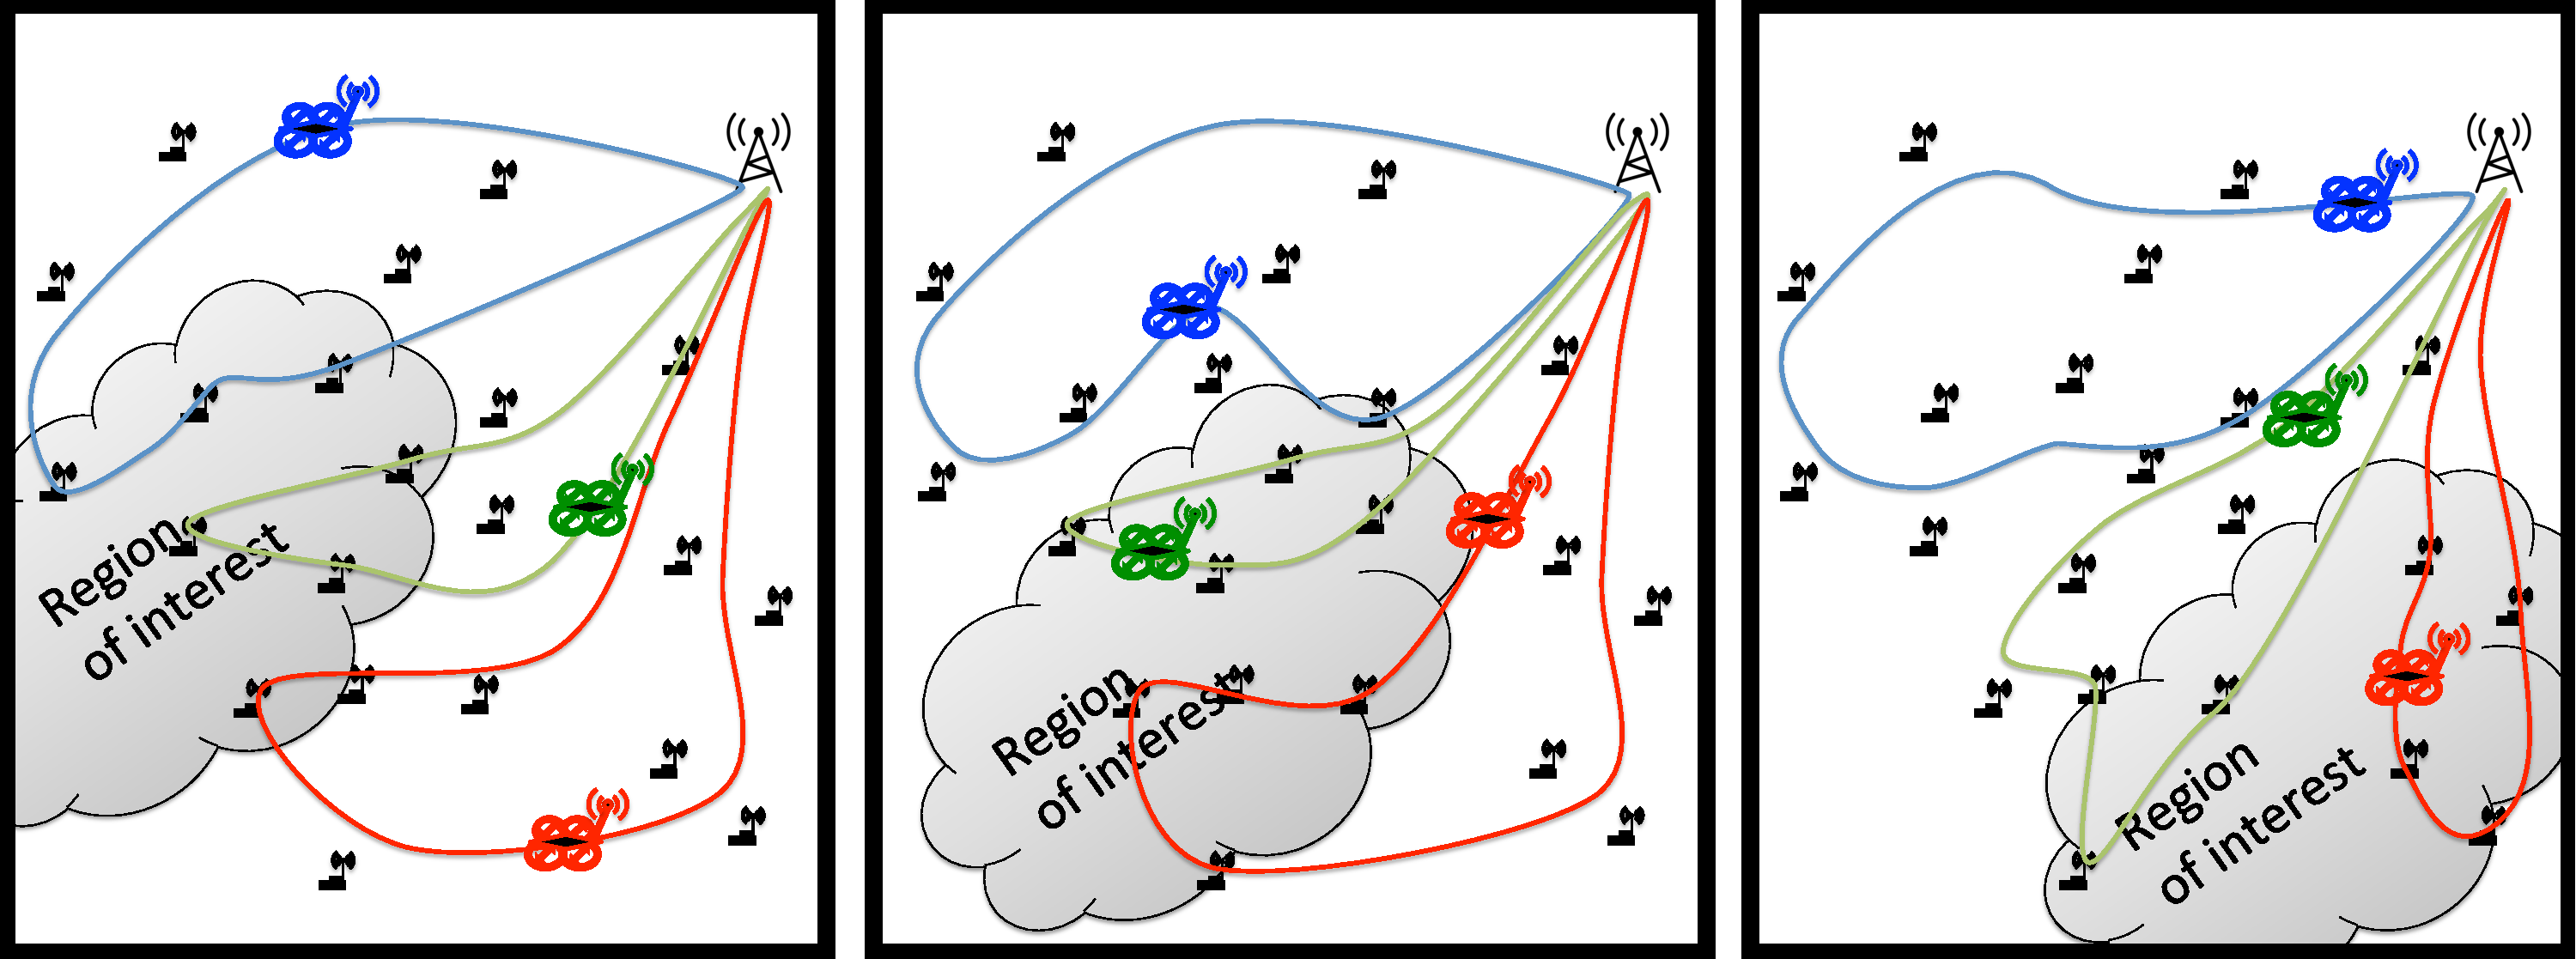
\includegraphics[width=\columnwidth]{dynamicVsStatic.pdf}
 % \end{center}
  %\vspace{-10pt}
  %\hspace{-35pt}
  \caption{\label{fig:dynamicVsStatic}The grey cloud represents a time-varying region of interest. Allowing the UVs to dynamically modify their routes in a distributed manner enables a robust response to changing conditions while maintaining service.}
\end{figure}

%\begin{figure}\centering
%  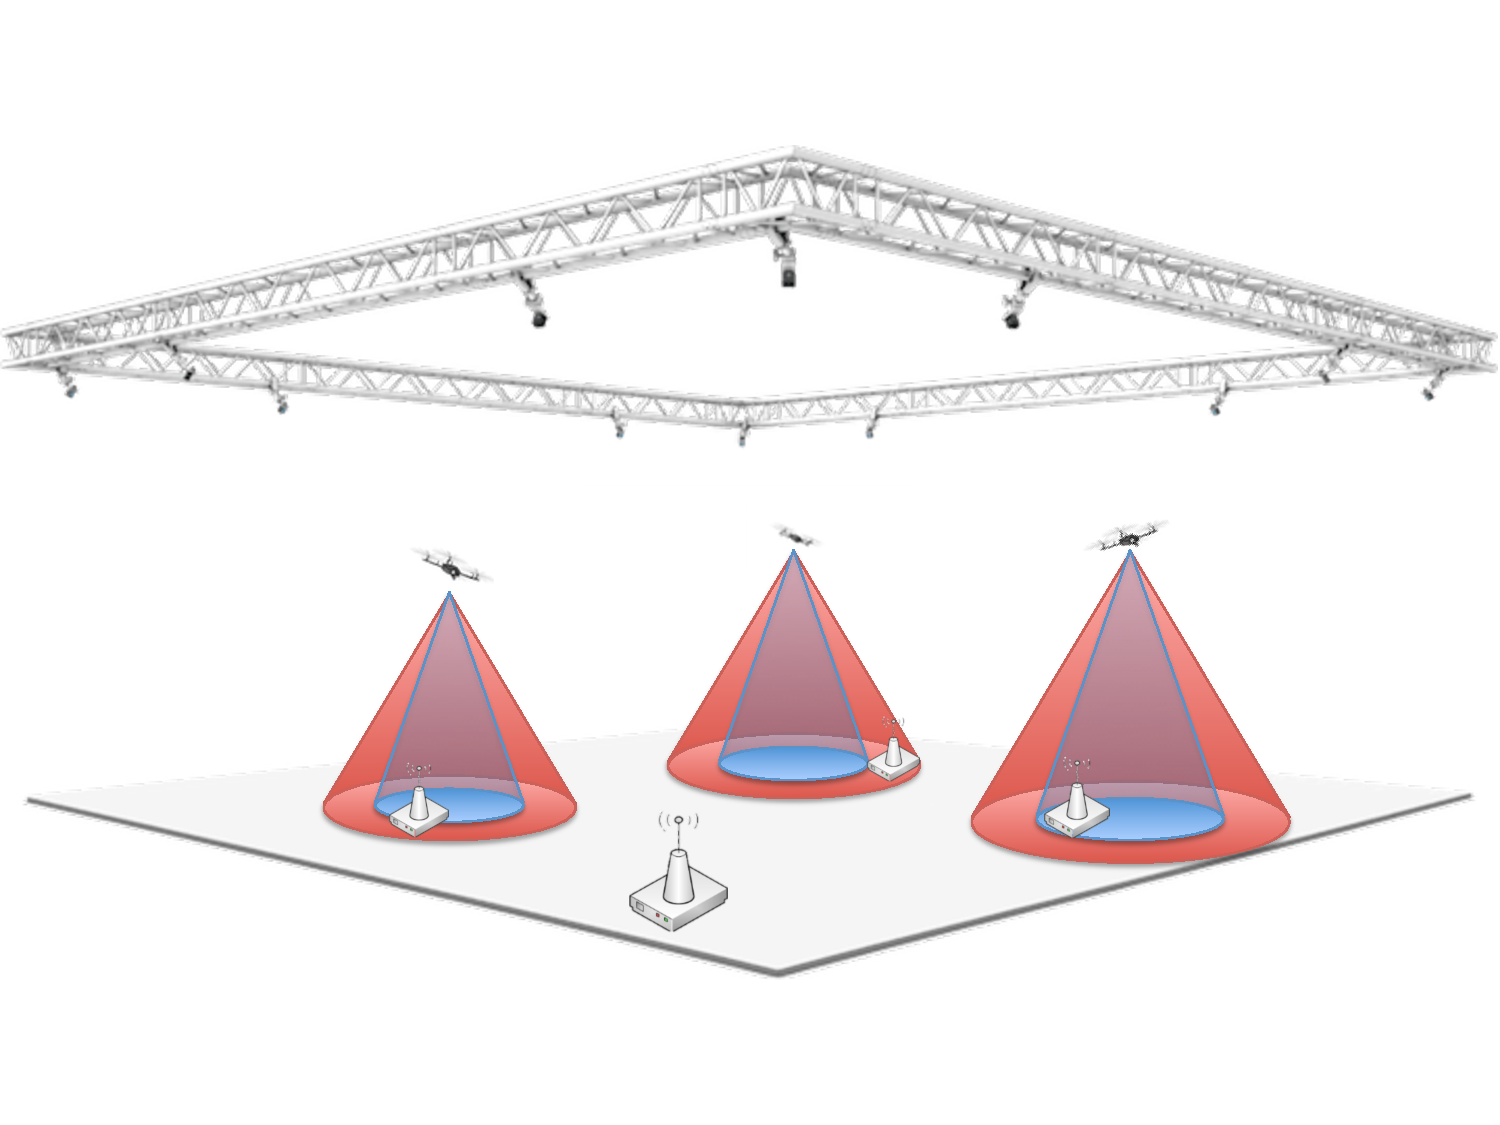
\includegraphics[width=\columnwidth]{hardwareTestbed3}
%\caption{Quadcopter testbed under construction for research on %recharging sensor nodes.\label{fig:QuadcopterTestbed}}
%\end{figure}

% use section* for acknowledgement
%\section*{Acknowledgment}
%The authors would like to thank...

\bibliography{./bibs/CySEES_ref,./bibs/zhu_ref,./bibs/ref,./bibs/Dissertation_reference_lanchao_C,./bibs/Match}

% that's all folks
\end{document}


